\documentclass[14pt,aspectratio=169,xcolor=dvipsnames]{beamer}
\usetheme{SimplePlus}
\usepackage{booktabs}
\usepackage{minted}

\title[short title]{Clase 10: Python científico}
\subtitle{}
\author[NA Barnafi] {Nicolás Alejandro Barnafi Wittwer}
\institute[UC|CMM] 
{
    Pontificia Universidad Católica de Chile \\
    Centro de Modelamiento Matemático
}

\titlegraphic{
    \vspace{-1.8cm}
    \begin{flushright}
      
\includegraphics[height=2.5cm]{../images/logos/puc.png} 
    \end{flushright}
}

\date{11/09/2024}
%\setbeamercovered{transparent}

\begin{document}
%%%%%%%%%%%%%%%%%%%%%%%%%%%%%%%%%%%%%%%%%%%%%%%%%%%%%%%
\begin{frame}
    \maketitle
\end{frame}
%%%%%%%%%%%%%%%%%%%%%%%%%%%%%%%%%%%%%%%%%%%%%%%%%%%%%%%
\begin{frame}[fragile]\frametitle{Motivación}
    \begin{itemize}
        \item Python es interpretado $\to$ lento
        \item Pero Python usa librerías \emph{MUY rápidas}
        \item Eso + sintaxis lo vuelven ideal para la ciencia
    \end{itemize}
    \begin{center}
    
\includegraphics[width=0.35\textwidth]{../images/baby-yoda-T.jpg} \hspace{1cm}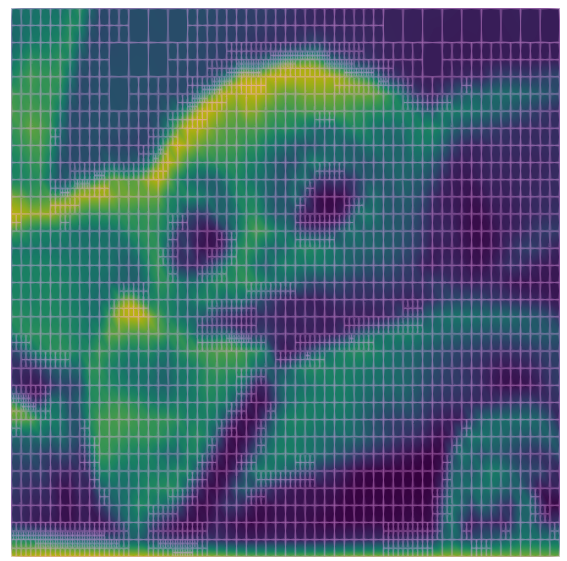
\includegraphics[width=0.35\textwidth]{../images/baby-yoda-mesh.png}
    \end{center}
\end{frame}
%%%%%%%%%%%%%%%%%%%%%%%%%%%%%%%%%%%%%%%%%%%%%%%%%%%%%%%
\begin{frame}[fragile]\frametitle{\texttt{math}}
    \begin{minted}{python}
  > import math
  > math. # Tab
math.acos(   math.copysign(  math.expm1(      math.lgamma(     math.pi          math.tanh(
math.acosh(  math.cos(       math.fabs(       math.log(        math.pow(        math.tau
math.asin(   math.cosh(      math.factorial(  math.log10(      math.prod(       math.trunc(
math.asinh(  math.degrees(   math.floor(      math.log1p(      math.radians(    math.ulp(
math.atan(   math.dist(      math.fmod(       math.log2(       math.remainder(  
math.atan2(  math.e          math.frexp(      math.modf(       math.sin(        
math.atanh(  math.erf(       math.fsum(       math.nan         math.sinh(       
math.ceil(   math.erfc(      math.gamma(      math.nextafter(  math.sqrt(       
math.comb(   math.exp(       math.gcd(        math.perm(       math.tan(  
    \end{minted}
    
\end{frame}
%%%%%%%%%%%%%%%%%%%%%%%%%%%%%%%%%%%%%%%%%%%%%%%%%%%%%%%
\begin{frame}\frametitle{NumPy}
    \textbf{Num}erical \textbf{Py}thon
    
    \begin{itemize}
        \item Permite hacer operaciones a grandes datos
        \item Operaciones \emph{vectorizadas}
        \item Submódulos útiles: 
            \begin{itemize}
                \item numpy.fft (Fourier transform)
                \item numpy.linalg (Linear algebra)
                \item numpy.polynomial (Polinomios)
                \item numpy.random (Generador de números)
            \end{itemize}
    \end{itemize}
\end{frame}
%%%%%%%%%%%%%%%%%%%%%%%%%%%%%%%%%%%%%%%%%%%%%%%%%%%%%%%
\begin{frame}[fragile]\frametitle{Numpy arrays}
    \begin{minted}{python}
  > import numpy as np
  > # 50 números equiespaciados en [0,1]
  > num = np.linspace(0,1,50)
  > # Números en [0,1) con paso 0.1
  > num = np.arange(0,1,0.1)
    \end{minted}

\pause \idea{Veamos tiempos de ejecución en sumar}
\end{frame}
%%%%%%%%%%%%%%%%%%%%%%%%%%%%%%%%%%%%%%%%%%%%%%%%%%%%%%%
\begin{frame}[fragile]\frametitle{Operaciones vectorizadas}
    $$ \text{vector:} \qquad x\in \mathbb{R}^N \to \left.\begin{bmatrix} 1\\1.1\\\vdots \\ -0.1\end{bmatrix}\right\}\text{N números} $$

    \begin{minted}{python}
  > import numpy as np
  > num = np.linspace(0,1,50)
  > np.abs(num) # Val absoluto de todo
  > np.exp(num) # exponencial
  > np.sin(num) # seno, ... etc
  > num.dot(num) # normas, producto interno, etc
    \end{minted}

\end{frame}
%%%%%%%%%%%%%%%%%%%%%%%%%%%%%%%%%%%%%%%%%%%%%%%%%%%%%%%
\begin{frame}\frametitle{Matplotlib}
    \centering
    \only<1>{
    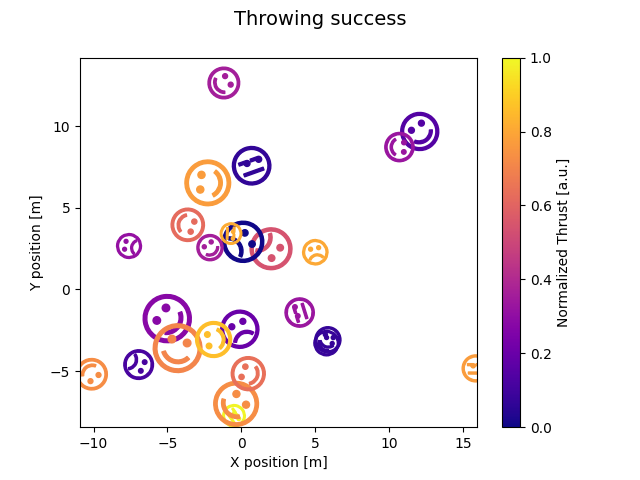
\includegraphics[width=0.6\textwidth]{../images/matplotlib/faces.png}
    }
    \only<2>{
    
\includegraphics[width=0.5\textwidth]{../images/matplotlib/mandelbrot.png}
    }
    \only<3>{
    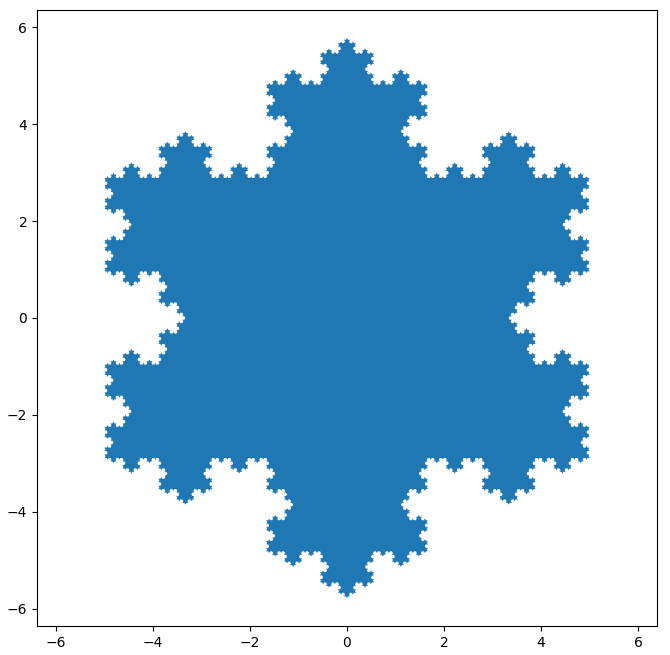
\includegraphics[width=0.5\textwidth]{../images/matplotlib/polygon.png}
    }
    \only<4>{
    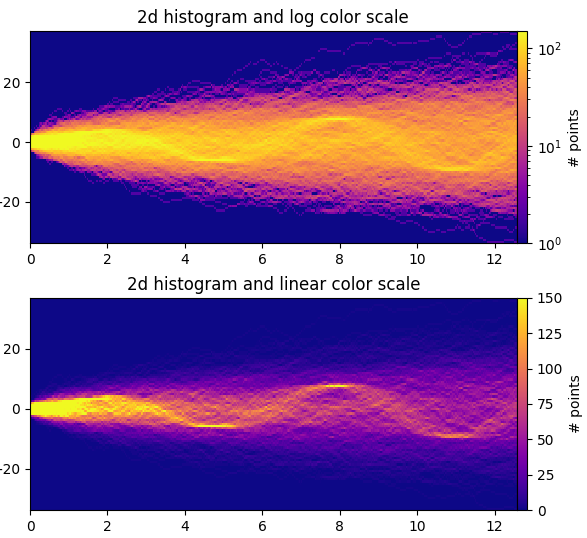
\includegraphics[width=0.5\textwidth]{../images/matplotlib/time-series.png}
    }
    \only<5>{
    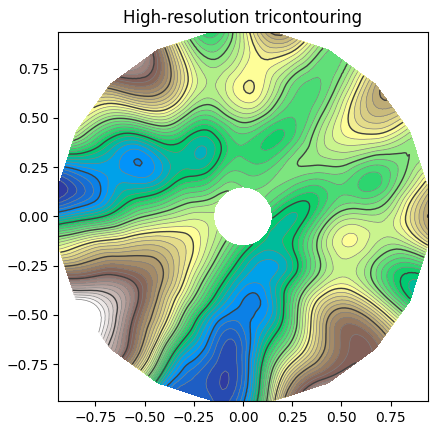
\includegraphics[width=0.5\textwidth]{../images/matplotlib/tricontourf.png}
    }
    \only<6>{
    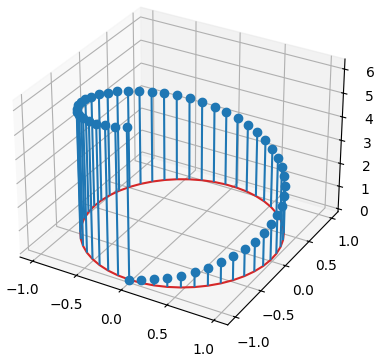
\includegraphics[width=0.5\textwidth]{../images/matplotlib/3dstem.png}
    }
    \only<7>{
    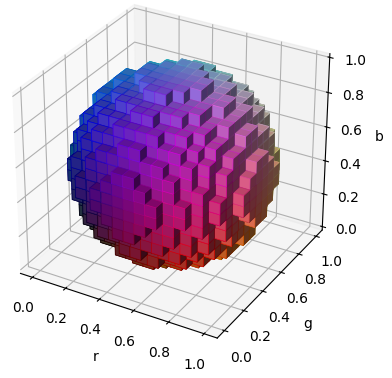
\includegraphics[width=0.5\textwidth]{../images/matplotlib/3dvoxel.png}
    }
\end{frame}
%%%%%%%%%%%%%%%%%%%%%%%%%%%%%%%%%%%%%%%%%%%%%%%%%%%%%%%
\begin{frame}[fragile]\frametitle{Ejemplo simple}
    \begin{minted}{python}
  > import numpy as np
  > import matplotlib.pyplot as plt
  > xs = np.linspace(0, 2*np.pi, 1000) # [0,2 pi]
  > ys = np.sin(xs)
  > plt.plot(xs,ys) # Lista de puntos x e y
  > plt.show()
    \end{minted} 
   
    \pause Se puede agregar de todo... 

    Ver documentación online: \texttt{matplotlib.org}.
\end{frame}
%%%%%%%%%%%%%%%%%%%%%%%%%%%%%%%%%%%%%%%%%%%%%%%%%%%%%%%
\begin{frame}\frametitle{Recap}
    \begin{itemize}
        \item \texttt{math}
        \item \texttt{Numpy}
        \item \texttt{Matplotlib}
    \end{itemize}
\end{frame}
%%%%%%%%%%%%%%%%%%%%%%%%%%%%%%%%%%%%%%%%%%%%%%%%%%%%%%%
\begin{frame}
    \maketitle
\end{frame}
%%%%%%%%%%%%%%%%%%%%%%%%%%%%%%%%%%%%%%%%%%%%%%%%%%%%%%%
\begin{frame}[fragile]\frametitle{Mini ejercicios}
    \begin{itemize}
        \item La función \code{time} del módulo \code{time} sirve para medir tiempo de ejecución. Compare el tiempo que se demora en sumar los primeros $N$ números en Python normal y luego con Numpy para $N$ creciente.
        \item Grafique los resultados en función del número de números total. Le podría servir \code{plt.semilogy}. 
    \end{itemize}
\end{frame}
%%%%%%%%%%%%%%%%%%%%%%%%%%%%%%%%%%%%%%%%%%%%%%%%%%%%%%%
\end{document}
